\newpage

\section{Dynamische Speicherverwaltung}

Mit den bisher eingeführten Grundlagen der Programmiersprache \texttt{C} kann man einfache Probleme lösen.
Das haben wir am Beispiel des Einfügesortierens gesehen.
Aber erst mit Hilfe dynamischer Speicherverwaltung und zusammengesetzter Datentypen kann man die volle Stärke von \texttt{C} ausnutzen.

\begin{figure}
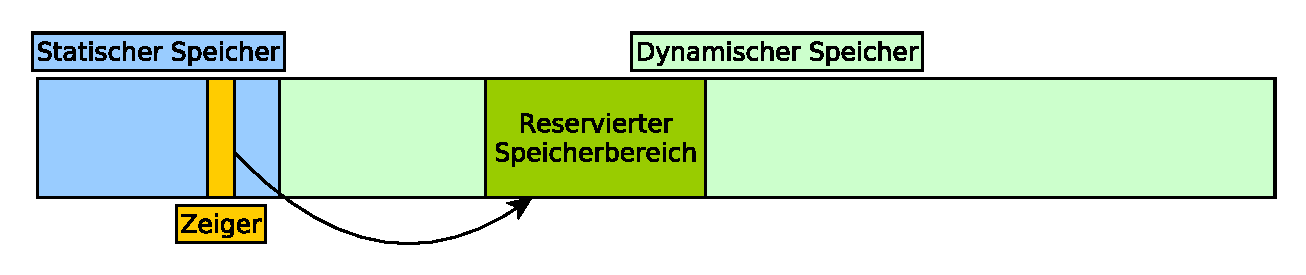
\includegraphics[width=\textwidth]{graphics/zeiger_auf_dynamischen_speicher}
\caption{\label{fig:abmem} Dynamischer und statischer Speicher eines Programms.}
\end{figure}

Bei der Benutzung von Arrays muss man immer schon zur Zeit der Übersetzung wissen, wie groß das Array maximal werden darf.
Das ist eine relativ starke Einschränkung, die sehr ineffizient sein kann.
Entweder, man hat viel zu viel Speicher bereitgestellt, oder zu wenig.
Genau passen wird es selten.

Der Speicher, der einem Programm zugeteilt ist, kann in zwei Kategorien unterteilt werden.
\begin{enumerate}
\item Statischer Speicher\\
  Dieses Teil haben wir schon kennengelernt. \index{Speicher!statisch}
  Im statischen Speicher befindet sich der Programmcode selbst, und der Speicher aller Variablen, die wir bisher deklariert haben.
  Seine Größe ist zum Zeitpunkt des Übersetzens festgelegt.

\item Dynamische Speicher\\
  Diesen Teil haben wir bisher noch nicht benutzt, aber jedes Programm kann eine bestimmte Menge an dynamischen Speicherplatz nutzen. \index{Speicher!dynamisch}
  Allerdings muss man sich zur Laufzeit des Programms selbst um das Reservieren und Freigeben dieses Speichers kümmern.
\end{enumerate}

Wenn wir also in einem Programm zum Beispiel einen Zeiger
\begin{lstlisting}
int *list;
\end{lstlisting}
deklarieren, so liegt dieser Zeiger selbst im statischen Speicherbereich.
Er kann aber auf Speicher zeigen, der im dynamischen Speicherbereich liegt.
Dies ist in Abbildung~\ref{fig:abmem} illustriert.

\subsection{Dynamische Speicherreservierung mit \texttt{malloc}}

\index{\texttt{malloc}}
Um Speicher dynamisch zu reservieren, nutzt man Funktionen aus der Standardbibliothek \verb|stdlib.h|.
Das Reservieren erledigt die Funktion \verb|malloc|, was für \emph{memory allocation} steht.
\verb|malloc| hat die folgenden Syntax:
\begin{mydefinitionblock}{Definition \texttt{malloc}}
  \begin{lstlisting}
    void *malloc(size_t size);
  \end{lstlisting}
  Reserviert Speicherzellen von der Größe \verb|size| bytes.
  \begin{itemize} 
    \itemsep0.2pt
  \item Rückgabewert: Wenn die Reservierung erfolgreich war, einen Zeiger auf den Anfang des
    reservierten Speicherbereiches, andernfalls \verb|NULL|.
  \item Eingabeparameter \verb|size|: die Größe des zu reservierenden Speicherbereiches in bytes.
  \item Beispielcode:
    \begin{lstlisting}
      int *array = (int *)malloc(sizeof(int) * 10);
    \end{lstlisting}
  \end{itemize}
  Man beachte, dass der reservierte Speicherbereich mit der Funktion \verb|free| (siehe unten) wieder freigegeben werden muss, wenn er nicht mehr benötigt wird. 
  Ansonsten steht er für das Programm nicht mehr zur Verfügung.
  Am Ende des Programms wird aller vom Programm reservierte Speicher automatisch freigegeben.
\end{mydefinitionblock}
Wir haben schon den Rückgabewert \verb|void| kennengelernt, der für keinen Rückgabewert steht.
Ein Zeiger auf \verb|void| repräsentiert einen Zeiger ohne Typ.\index{\texttt{void}}\index{Zeiger!\texttt{void}}
Er kann bzw. muss später mit einem \emph{cast} in jeden anderen Zeigertyp umgewandelt werden.
Deshalb wird im Beispielcode ein expliziter \emph{cast} nach \verb|int *| durchgeführt, den man immer bei der Benutzung von \verb|malloc| machen sollte.

Den Zeiger \verb|NULL| haben wir schon kennengelernt. \index{Zeiger!\texttt{NULL}}
\verb|malloc| gibt \verb|NULL| zurück, falls das Reservieren aus irgendeinem Grund nicht erfolgreich war.
Daher ist es sehr wichtig bei jedem Aufruf von \verb|malloc| den Rückgabewert auf \verb|NULL| zu testen!
Die Größe eines Typs in byte liefert die Funktion \verb|sizeof|.

\subsection{Speicherfreigabe mit \texttt{free}}

\index{\texttt{free}}
Wie schon angedeutet, dynamisch reservierter Speicher muss wieder freigegeben werden, wenn er nicht mehr benötigt wird.
Dafür gibt es die Funktion \verb|free|:
\begin{mydefinitionblock}{Funktion Definition \texttt{free}}
  \begin{lstlisting}
    void free(void *memory);
  \end{lstlisting}
  Gibt einen mit \verb|malloc| reservierten Speicherbereich wieder frei.
  \begin{itemize}
  \item Eingabeparameter: Zeiger auf einen Speicherbereich, der mit \verb|malloc| reserviert wurde.
  \item Beispiel:
    \begin{lstlisting}
      int *array = (int *)malloc(sizeof(int) * 10);
      free(array);
    \end{lstlisting}
  \end{itemize}
\end{mydefinitionblock}
Wendet man \verb|free| auf einen Zeiger an, der nicht auf den Anfang eines mit \verb|malloc| reservierten Bereiches zeigt, so erhält man einen Laufzeitfehler.

\subsection{Mehrdimensionale Arrays}

Bisher haben wir uns auf eindimensionale Arrays beschränkt.
Als Beispiel für ein mehrdimensionales Array betrachten wir eine Drehmatrix in zwei Dimensionen um den Winkel $\alpha$. \index{Feld!mehrdimensional}
Es handelt sich um eine lineare Abbildung, die einen zweidimensionalen Vektor $(x,y)^t$ auf den Vektor $(x',y')^t$ wie folgt abbildet:
\begin{equation}
  \left(\begin{array}{c}x^{,}\\y^{,}\end{array}\right)=
  \left(\begin{array}{cc} \cos\left(\alpha\right) & \sin\left(\alpha\right) \\
    -\sin\left(\alpha\right) & \cos\left(\alpha\right) 
  \end{array}\right)
  \left(\begin{array}{c}x\\y\end{array}\right)
\end{equation}
Die entsprechende Matrix kann man in \texttt{C} mit Hilfe von zweidimensionalen Arrays darstellen.
Die Deklaration eines statische $2\times2$ Arrays sieht wie folgt aus:
\begin{lstlisting}
double rotate2d[2][2];
\end{lstlisting}
An Hand dieser Deklaration kann man mit dem jetzigen Vorwissen ahnen, dass ein zweidimensionales Array ein Array von Arrays ist.
Daher entspricht ein solches zweidimensionales Array auch einem Zeiger auf einen Zeiger auf einen Typ.
Diskutieren wir wieder ein Beispiel:
\begin{lstlisting}
#include <math.h>
#include <stdio.h>
#include <stdlib.h>
int main()
{
  const int SPACEDIM = 2;
  const double M_PI = 3.1415;

  // Speicher reservieren
  double **array2d;
  if ((array2d = (double **)malloc(sizeof(double *) * SPACEDIM)) == NULL)
    {
      printf("Fehler in malloc\n");
      return (-1);
    }
  for (int i = 0; i < SPACEDIM; ++i)
    {
      if ((array2d[i] = (double *)malloc(sizeof(double) * SPACEDIM)) == NULL)
        {
          printf("Fehler in malloc\n");
          return (-2);
        }
    }
  // Werte zuweisen
  array2d[0][0] = cos(M_PI / 4.);
  array2d[0][1] = sin(M_PI / 4.);
  array2d[1][0] = -sin(M_PI / 4.);
  array2d[1][1] = cos(M_PI / 4.);
  // Ausgabe
  for (int i = 0; i < SPACEDIM; ++i)
    {
      for (int j = 0; j < SPACEDIM; ++j)
        {
          printf("%e ", array2d[i][j]);
        }
      printf("\n");
    }
  // Speicher freigeben
  for (int i = 0; i < SPACEDIM; ++i)
    {
      free(array2d[i]);
    }
  free(array2d);
  return (0);
}
\end{lstlisting}
\verb|array2d| ist jetzt als \verb|double**| deklariert, also als Zeiger auf einen \verb|double| Zeiger. 
Dann wird zunächst Speicher für ein Array von \verb|double*| Zeigern reserviert.
Das geschieht in Zeile $10$.
Man beachte, wie an dieser Stelle der Rückgabewert von \verb|malloc| auf \verb|NULL| getestet wird.
Eine Zuweisung der Form \verb|(x = y)| hat selbst den Wert von \verb|x|.
Anschließend wird in der Schleife, die in Zeile $14$ anfängt, für jedes Element des Arrays von \verb|double*| Zeigern selbst wieder Speicher reserviert.
Das muss nun Speicher für \verb|double| selbst sein.
Wieder testen wir den Rückgabewert von \verb|malloc| auf \verb|NULL|.

Es ist wichtig, sich klar zu machen, dass \verb|array2d| vom Typ \verb|double**| ist.
Dementsprechend zeigt es auf Elemente vom Typ \verb|double*|, die dann selbst auf Elemente vom Typ \verb|double| zeigen.
Dies ist in Abbildung~\ref{fig:mem2d} dargestellt.

\begin{figure}[!ht]
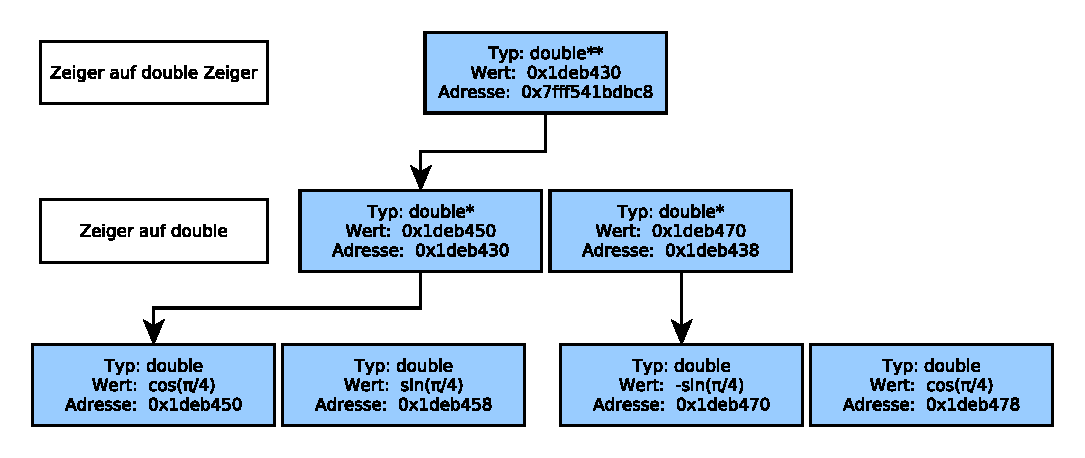
\includegraphics[width=\textwidth]{graphics/zeiger_auf_zeiger}
\caption{Illustration Zeiger auf Zeiger. \label{fig:mem2d}}
\end{figure}

Es bietet sich an für die Speicherreservierung einer zweidimensionalen Matrix eine eigene Funktion zu schreiben.
Es ist schließlich ziemlich wahrscheinlich, dass mehr als eine solche Matrix benötigt wird.
Der entsprechende Quelltext könnte beispielsweise so aussehen:
\begin{lstlisting}
#include <math.h>
#include <stdio.h>
#include <stdlib.h>

double **create2darray(const int dim)
{
  double **p1 = NULL;
  if ((p1 = (double **)malloc(sizeof(double *) * dim)) == NULL)
    {
      return (NULL);
    }
  for (int i = 0; i < dim; ++i)
    {
      if ((p1[i] = (double *)malloc(sizeof(double) * dim)) == NULL)
        {
          return (NULL);
        }
    }
  return (p1);
}

int main()
{
  const int SPACEDIM = 2;
  const double M_PI = 3.1415;

  double **array2d;
  if ((array2d = create2darray(SPACEDIM)) == NULL)
    {
      printf("Fehler in malloc\n");
      return (-1);
    }
  // Zuweisen
  array2d[0][0] = cos(M_PI / 4.);
  array2d[0][1] = sin(M_PI / 4.);
  array2d[1][0] = -sin(M_PI / 4.);
  array2d[1][1] = cos(M_PI / 4.);
  for (int i = 0; i < SPACEDIM; ++i)
    {
      for (int j = 0; j < SPACEDIM; ++j)
        {
          printf("%e ", array2d[i][j]);
        }
      printf("\n");
    }
  // hier sollte noch der Speicher freigegeben werden!
  return (0);
}
\end{lstlisting}
Die Funktion \verb|create2darray| liefert als Rückgabewert eine Variable vom Typ \verb|double**|, also genau das, was wir benötigen.
In der Funktion selbst geschieht dann das, was wir im obigen Beispiel schon gezeigt hatten.
Mit \verb|return| wird dann das Objekt zurückgegeben, für das wir Speicher reserviert haben.

An dieser Stelle sieht man einen wichtigen Unterschied zwischen der Deklaration einer Variablen und dem Reservieren von Speicher mit \verb|malloc|.
Währen beispielsweise die Variable \verb|p1| in der Funktion \verb|create2darray| natürlich nur in der Funktion selbst sichtbar ist, bleibt der mit \verb|malloc| reservierte Speicher auch außerhalb der Funktion reserviert.
Und indem wir die Adresse zu dieser Speicherstelle von der Funktion an die aufrufende Funktion übergeben, können wir den reservierten Speicherbereich auch außerhalb der Funktion nutzen.

Das bedeutet aber auch, dass Speicher, der mit \verb|malloc| reserviert wurde, und dessen Adresse wir nicht mehr kennen, nicht mehr nutzbar ist.
Auf diese Art und Weise kann man recht einfach versehentlich Programme schreiben, die den gesamten Hauptspeicher eines Rechners reservieren, ohne ihn zu nutzen.
Das führt relativ schnell zur Unbenutzbarkeit des entsprechenden Rechners.
Ein Beispiel für einen solchen Fehler ist der folgende (nicht besonders sinnvolle) Code Abschnitt
\begin{lstlisting}
int list[50];
doubke *p;
for (int i = 0; i < 50; i++)
  {
    p = malloc(sizeof(double));
    *p = i * i;
    list[i] = *p + (*p) * (*p);
  }
free(p); // falsche Stelle!
\end{lstlisting}
In jedem Durchlauf der Schleife wird Speicher für \verb|p| reserviert, ohne ihn wieder frei zu geben.
Nach Ende der Schleife ist keine der Adressen all dieser Reservierungen (bzw. nur noch die letzte) mehr verfügbar.
D.h. man kann den Speicher weder weiter benutzen, noch kann man ihn nachträglich frei geben, ein Umstand der als Speicherleck oder \emph{memory leak} bezeichnet wird.

\endinput
